\documentclass[
  11pt,
  fleqn
]{article}
% [fleqn] left-aligns all equations

% fonts

\usepackage[T1]{fontenc} % Apparently this
% https://tex.stackexchange.com/questions/287312/font-not-loadable-metric-data-not-found-or-bad
\usepackage[full]{textcomp}
\usepackage[final,expansion=alltext,nopatch=footnote]{microtype}
\usepackage{csquotes} % suppress warning from `babel`
\usepackage[english]{babel}
\usepackage[fleqn]{mathtools}
\usepackage[cal=boondoxo]{mathalpha} % mathcal

\usepackage{amsthm} % gives proof environment:
% https://www.overleaf.com/learn/latex/Theorems_and_proofs

\usepackage{newtxtext}
% \usepackage{txfonts} % See
% https://tex.stackexchange.com/questions/444243/symbols-not-showing-up

% These need to be after newtxtext
\usepackage[varqu,varl]{inconsolata} % sans serif typewriter
% \usepackage{cabin} % sans serif - ugly

\usepackage[bigdelims,vvarbb]{newtxmath} % bb from STIX % "should be
% loaded AFTER the text font" -
% https://mirrors.mit.edu/CTAN/fonts/newtx/doc/newtxdoc.pdf

% geometry of the page

\usepackage[
  % top=1in,
  % bottom=1in,
  % left=1in,
  % right=1in
]{geometry}

% paragraph spacing

\setlength{\parindent}{0pt}
\setlength{\parskip}{1.5ex plus 0.4ex minus 0.2ex}

% useful packages

% \usepackage{natbib} % incompatible with BibLaTeX
\usepackage{epsfig}
\usepackage{url}
\usepackage{bm}
\usepackage{blindtext}

% Leon additions

\usepackage{enumitem} % allows for enumerate[resume]

\usepackage{booktabs}

\usepackage[
  style=authoryear-comp,
  natbib=true,
  % refsection=chapter,
  url=false,
  doi=true,
  isbn=false,
  date=year %
  % https://tex.stackexchange.com/questions/55780/disable-month-in-biblatex-bibliography
]{biblatex} % natbib=true allows \citep
% Clear "visited on"
% https://tex.stackexchange.com/questions/400384/how-to-disable-biblatex-showing-visited-on-on-the-references
\AtEveryBibitem{
  \clearfield{urlyear}
  \clearfield{urlmonth}
  \clearfield{eprint} % remove PMID %
  % https://tex.stackexchange.com/questions/250784/removing-eprint-and-eprinttype-in-citation-notes
}

\usepackage{graphicx}
% ensures figures stay in their section
% https://tex.stackexchange.com/questions/279/how-do-i-ensure-that-figures-appear-in-the-section-theyre-associated-with
\usepackage[section]{placeins}

% Section formatting using titlesec
\usepackage{titlesec}
\titleformat*{\section}{\singlespacing\sffamily\Large}
\titleformat*{\subsection}{\singlespacing\sffamily\large}
% \titleformat*{\subsubsection}{\itshape}
\titleformat*{\paragraph}{\itshape}
\titleformat{\chapter}{\singlespacing\sffamily\Huge}{{\thechapter}}{1em}{}

% center figures by default
\makeatletter
\g@addto@macro\@floatboxreset\centering
\makeatother
% italic figure captions
\usepackage[format=plain,
  textfont=it,
]{caption}

% simple TO DO and comment macros
\usepackage[
  % https://tex.stackexchange.com/questions/4503/how-do-i-specify-color-in-rgb-using-hypersetup-in-hyperref
  dvipsnames,svgnames,x11names
]{xcolor}
\newcommand\todo[1]{\textcolor{orange}{[#1]}}% simple TO DO macro
\newcommand\comment[1]{\textcolor{red}{[#1]}}

\usepackage{url}
\usepackage[
  hidelinks,
  pdfa % Required for valid pdf/a output:
  % https://tex.stackexchange.com/questions/431022/pdf-a-validation-problem-the-f-key-is-missing
]{hyperref}
\hypersetup{
  % colorlinks,
  % linkcolor=RoyalBlue4,
  % citecolor=PaleVioletRed4,
  % urlcolor=Firebrick4
}

\newcommand{\indsim}{\overset{\mathrm{ind}}{\sim}}
% https://tex.stackexchange.com/questions/60545/should-i-mathrm-the-d-in-my-integrals
\newcommand*\diff{\mathop{}\!\mathrm{d}}
\newcommand*\Diff[1]{\mathop{}\!\mathrm{d^#1}}
\newcommand{\e}{\mathrm{e}}
\newcommand{\E}{\mathrm{E}}
\renewcommand{\P}{\mathrm{P}}
\newcommand{\N}{\mathrm{N}}
\newcommand{\diag}{\mathrm{diag}}
\newcommand{\ave}{\mathrm{ave}}
\newcommand{\Var}{\mathrm{Var}}
\newcommand{\Cov}{\mathrm{Cov}}
\newcommand{\cov}{\mathrm{cov}}
\newcommand{\sd}{\mathrm{sd}}
\newcommand{\var}{\mathrm{var}}
\newcommand{\corr}{\mathrm{corr}}
\renewcommand\vec{\boldsymbol}

% Overlap-specific
\newcommand{\rank}{R}
\newcommand{\rmax}{m}
\newcommand{\rgap}{r^\text{gap}}
\newcommand{\Ngap}{N_1^\text{gap}}
\newcommand{\pigap}{\pi_1^\text{gap}}

% For appearance of block matrices
% https://tex.stackexchange.com/questions/495903/horizontal-and-vertical-lines-in-pmatrix
\renewcommand{\arraystretch}{1.5}

% Theorem-type environments
\newtheorem{definition}{Definition}[section]
\newtheorem{result}[definition]{Result}
\newtheorem{claim}[definition]{Claim}

% From Datta template
% https://github.com/bibekanandadatta/JHU-Dissertation-Template

\usepackage{setspace}                         % sets space between lines

%%%% JH Library requirement (DO NOT CHANGE)
\def\GlobalMargin{1.0in}                      % margin on all sides
% \def\PrintingOffset{0.5in}                  % additional left
% margin for the printed copy
\def\PrintingOffset{0.0in}
\def\MainTextSpacing{\singlespacing}        % double-spaced main text
% \def\MainTextSpacing{}
\def\CaptionStretch{1.1}                    % to match 2x spacing
% \def\CaptionStretch{1.0}

\captionsetup{font={stretch=\CaptionStretch}}

\geometry{
  letterpaper,
  margin=\GlobalMargin,
  bindingoffset=\PrintingOffset,
  nomarginpar,
  % includehead,
  % headheight=\HeaderHeight,
  % headsep=\HeaderSpace,
  includefoot,
  heightrounded
}

%%%% BIBLIOGRAPHY ITEMS
\def\BibTextSpacing{\onehalfspacing}         % single-spaced bibliography
% \def\BibTextSpacing{\singlespacing}         % single-spaced bibliography
\def\BibItemSpacing{\baselineskip}          % spacing between
% bibliographic items in reference

%%%% UNNUMBERED CHAPTERS, SECTION, and SUBSECTION COMMAND for ADDING to TOC
%% removes the 'Chapter #' title while keeping it listed in the TOC
\newcommand\chap[1]{%
  \chapter*{#1}%
  \markboth{#1}{}
\addcontentsline{toc}{chapter}{#1}}

%% removes the 'Section #' title while keeping it listed in the TOC
\newcommand\sect[1]{%
  \phantomsection
  \section*{#1}%
\addcontentsline{toc}{section}{#1}}

%% removes the 'Subsection #' title while keeping it listed in the TOC
\newcommand\subsect[1]{%
  \phantomsection
  \subsection*{#1}%
\addcontentsline{toc}{subsection}{#1}}

%% removes the 'Subsubsection #' title while keeping it listed in the TOC
\newcommand\subsubsect[1]{%
  \phantomsection
  \subsubsection*{#1}%
\addcontentsline{toc}{subsubsection}{#1}}

% Correct matrix for double spacing
% https://tex.stackexchange.com/questions/137004/matrix-within-equation/137009#137009
\makeatletter
\def\env@matrix{\hskip -\arraycolsep
  \let\@ifnextchar\new@ifnextchar
  \linespread{1}\selectfont
  \renewcommand{\arraystretch}{1.2}%
\array{*\c@MaxMatrixCols c}}
\makeatother

% Footnotes must be 2 points less than main text but larger than 8pt
\usepackage{footmisc}
\renewcommand{\footnotesize}{\fontsize{9pt}{11pt}\selectfont}

% For including CV
\usepackage{pdfpages}

% Generate PDF/A (archival format)
% https://webpages.tuni.fi/latex/pdfa-guide.pdf
\usepackage[a-1b,mathxmp]{pdfx}

\usepackage[
  nottoc % Don't include TOC in TOC
]{tocbibind}

% Redefine `abstract`s so they can be at the start of each chapter
% don't cause the page numbering to reset
% https://tex.stackexchange.com/a/4857
\newenvironment{myAbstract}{
  \rightskip.5in
  \leftskip.5in
  % \itshape
}{}

% For writing/planning purposes: show paragraph level in TOC
\setcounter{secnumdepth}{2}

\addbibresource{bibliography.bib}
\graphicspath{{fig/}}

\title{Advice on developing ordinal outcomes and endpoints for clinical trials}
\author{Leon Di Stefano, Katherine Lee, etc\ldots}
\date{\today}

\begin{document}

\maketitle

\tableofcontents
\newpage

\section{Introduction}

Ordinal outcomes have become increasingly prominent in clinical
resarch, particularly following the COVID-19 pandemic.

Some advantages of ordinal outcomes are that they can
\begin{enumerate}
  \item Provide more information that binary outcomes, including
    composite outcomes, allowing for more efficient and ethical studies
  \item Allow for the incorporation of safety events into one's
    primary outcome and therefore account for many different aspects
    of benefit/harm. At the same time, they do not require a
    fully-specified utility function (which may differ from patient
    to patient or require more extensive development and validation)
  \item Allow for the combination of discrete and continous outcome
    measures (for example a numerical quality of life scale with
    death as the worst outcome)
  \item Allow for the incorporation of intercurrent events into one's
    primary outcome, avoiding complexities of alternative estimand strategies
    like principal stratum estimands (particular for truncating
    events like death) while having more statistical efficiency than
    binary composite estimands (see point (1))
\end{enumerate}

The goal of this manuscript is to serve as a guide for clinicians and trialists
in choosing/developing ordinal outcomes for their studies. We consider both
both the outcome itself (the data recorded on each patient) and effect
measures or ``endpoints'' (the metric used to compare patient groups).

We want to distinguish \emph{choosing} an outcome/effect measure from
\emph{validating} the outcome/effect measure using external data. This paper is
about the first task, choosing (or constructing) the outcome and effect
measure. In practice choosing an outcome and effect measure and validating that
outcome and effect measure in pre-trial data will be an iterative process; our
focus is on the ``positive'' side of the process, namely coming up
with, and tweaking, proposed outcomes and effect measures.

\section{Desiderata for outcomes and effect measures}

We want outcomes that
\begin{enumerate}
  \item reflect patient benefit and harm
  \item capture sufficient information to efficiently discriminate
    among better- and
    worse-off patients.
\end{enumerate}

We want effect measures that
\begin{enumerate}
  \item capture decision-relevant differences in distributions of
    patient benefit and harm
  \item are easy to interpret and to translate into practical recommendations
\end{enumerate}

\section{Techniques for constructing ordinal outcomes}

\subsection{Tie-breaking can be used to combine and fine-grain ordinal outcomes}

Two basic operations:
\begin{enumerate}
  \item Complete tie-breaking of $A$ by
    $B$ (lexicographic order)
  \item Tie-breaking of $A$ by $B$ \emph{within a
    specific level $a$ of $A$} (equivalently, ``overriding'' $B$ by $A$) is the
    combination of these.
\end{enumerate}

Tie breaking within a level (2) is a combination of complete
tie-breaking (1) and merging.

\subsubsection{Incorporating longitudinal or time-to-event information}

Distinguish between ``state'' and ``trajectory'' variables. State
variables summarize patient outcomes at a particular moment in time.
Trajectory variables, including times-to-event, summarize patient
state over a timecourse.

Trajectory variables can be incorporated into an ordinal outcome. For example
(from PASSPORT) ``worst pSOFA while hospitalized until day 28''.

Incorporating trajectory variables into an ordinal outcome may seem unnatural.
But arguable most existing time-to-event analyses are in fact analyses of an
ordinal outcome. The Cox model for time-to-event data treats time as ordinal:
because (1) the baseline hazard is not modelled, (2) the model itself is
invariant to monotone rescalings of the time axis, and (3) the (partial)
likelihood (ignoring ties) depends only on the ranks of the data (i.e., is a
marginal likelihood). The Cox model is essentially an ordinal
stopping ratio model with complementary log-log link. (Perhaps a
difference is censoring.)

\subsection{Coarsening (composite outcomes) can be used to avoid
directly comparing levels}

This comes from the experience of presenting the PASSPORT outcome:
clinicians thought that including, for example, "digit amputation
before day 28" and "ECMO before day 28" within the same level of an
ordinal outcome meant assuming that the two outcomes have the
\emph{same} utility. In fact it represents \emph{refusing to compare}
their utilities.

\subsection{Category probabilities affect precision and power mostly via the
probability of the largest category}

Theory of \citep{} says that the relative efficiency (variance) of an
unadjusted treatment comparison using an ordinal versus continuous outcome in
the proportional odds model is given by $1 - \sum \overline p_c^3$ where
$\overline p_c$ is the marginal probability (averaged over control and
experimental groups) of outcome category $c$.

Efficiency is maximized at $1 - 1/C^2$ where $C$ is the total number of
categories when the probabilities are all equal: $\overline p_c = 1/C$.

We have simulation results and some math to show that the value of $\sum_c
\overline p_c^3$ is \emph{essentially a function of the largest category
probability} $\overline{p_{\max}} = \max \overline{p_c}$. See \ref{fig:p_max}
for an illustration.

\begin{figure}
  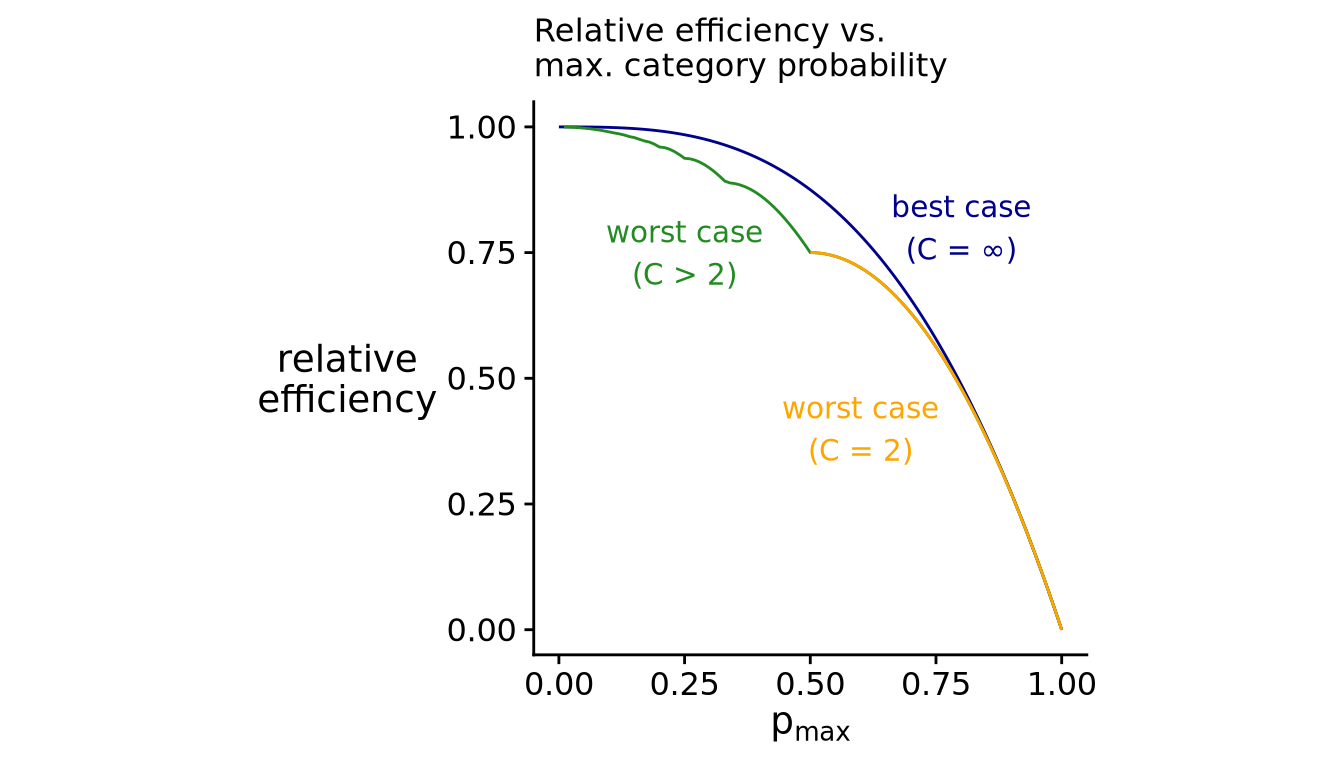
\includegraphics[width=6in]{p_max_controls_efficiency.png}
  \caption{Bounds on the relative efficiency of an ordinal outcome
    compared to its continuous counterpart as a function of the maximum
  category probability.}
  \label{fig:p_max}
\end{figure}

Thus simple advice is: for statistical efficiency, try to make the proportion
of patients in the largest category small.

\section{Guidelines for choosing estimands or effect measures}

The basic problem: we want to compare two distributions (control and
experimental groups) over ordinal outcomes with a single number.

In general this represents a loss of information. Let's say the
outcome has $L$ levels. Then the distributions in each
arm is specified by $L-1$ numbers (for the first $L-1$ probabilities,
  or cumulative logits, or stopping ratio logits--reflecting the
sum-to-1 constraint on probability distributions) and so the
\emph{difference} between the distributions is also specified by
$L-1$ numbers (for example the differences between the cumulative
logits, or logit stopping probabilities).

An effect measure thus represents a way to collapse these $L-1$
numbers into one.

\subsection{Model-based effect measures}

Model-based: common odds ratio; common stopping ratio or common continuation
ratio.

What they have in common: the effect measure is a byproduct of fitting a model
to the data. The model typically assumes that a certain pattern holds in the
outcome distributions across groups so that the differences in distributions
can be described by a single number (with more than two groups, $G-1$ numbers).

\subsection{Model-free effect measures}

Nonparametric or model-free measures: probabilistic index, win ratio, win odds,
etc.

\subsubsection{Connection with win win/generalized pairwise comparison
methods}

Win/generalized pairwise comparison methods are implicitly about (1)
constructing ordinal outcomes through tie-breaking (2) in a way that is
compatible with right-censoring (3) estimating nonparametric effect
measures (4) defining comparisons of two distributions by averaging
over draws from the distributions as if they were independent
(pairwise comparisons).

\subsection{Comparing model-based and nonparametric effect measures}

Both of these can be considered ``estimands'', insofar as we consider
the model-based effect measures to be defined by the estimate from
the best-fitting model in the population.

Nonparametric effect measures may appear to be assumption-free. However

\begin{itemize}
  \item Assumptions don't need to hold exactly for the model-based
    effect measures to make sense
  \item The model-free methods also may not make sense, if for
    example there are nonmonotone effects across cutpoints
  \item Model-free methods don't define a common scale for comparing
    more than two interventions. For example, model-free effect
    measures can be nontransitive
  \item Model-based methods have additional advantages, for example
    the possibility of adjustment for covariates.

    When additivity approximately holds, this yields a ``best of both
    worlds'' effect measure that is
    personalized effect measure that is yet reportable as a single
    number.
\end{itemize}

Simulations show a typically very strong association between
proportional odds ratios and probabilistic indices [cite Harrell].

Reducing to a composite binary outcome
\begin{itemize}
  \item Based on a specific cutpoint, e.g. ``hospitalization or worse''
  \item Based on a quantile in a reference group; for example,
    ``worse than the median outcome under standard care''
\end{itemize}

One point of view is that one would ``ideally'' analyze ordinal
outcomes by reporting the associated expected utilities [cite Berry
talk; example of utility-weighted Rankin scale].

We should distinguish between effect measures used for
\emph{analysis} and for \emph{reporting}. It may make sense to report
the probabilistic index even if the analysis is undertaken using a
proportional odds model.

\section{Conclusions}

\end{document}
